\chapter{Caching Basics}
\label{chapter:caching-model}

In order to get a common understanding of caching and the terminology related to the topic, we will give a brief introduction to the basics of caching by describing a basic caching algorithm and the common caching architecture. The chapter also introduces the timeline model used to visualize how a caching approach works, and presents a set of criteria used to evaluate caching approaches.

\section{Basic Caching Algorithm}
\label{sec:caching_basics}

In general caching is about storing the result of a computation, such that it for future requests is possible to get the result fast instead of recomputing it. This basic algorithm is described on figure~\ref{fig:basic-caching}.

\begin{figure*}[ht!]
  \begin{center}
    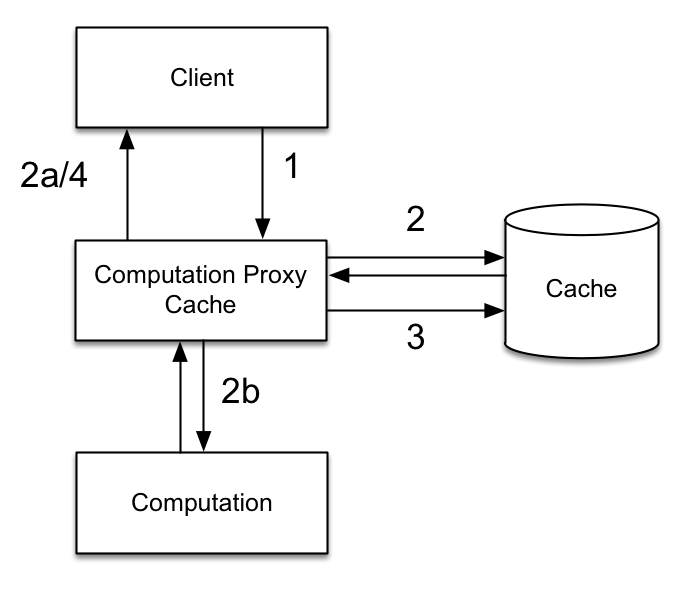
\includegraphics[width=0.6\linewidth]{figures/basic-caching-figure.pdf}
  \end{center}
  \begin{enumerate}
    \item The caller requests the value of the computation by calling the proxy
    \item The proxy fetches the cached value of the computation through the cache
    \item[(3)] The proxy calls the computation
    \item[(4)] The result of the computation is stored in the cache
    \item The value is returned to the caller
  \end{enumerate}
  \footnotesize{Steps annotated with \emph{parenthesis and dashed lines} are only executed in case of cache miss or cache failure.}
  \caption{The flow of basic caching}
  \label{fig:basic-caching}
\end{figure*}

If we look at the cached object from an abstract point of view, we can see it as a \emph{result of a function} given certain \emph{inputs}. Sometimes the inputs are data from a storage system, the result of an API call to some external resource, or maybe a global variable in the code. Some of these inputs are used to identify the cached function, but others change during the lifetime of the cached value. We call these changing input, \emph{underlying data}.

In order for the algorithm to work, we need to be sure that a cached object is uniquely identified by a given name. This presents one of the challenges of cache management, which involves naming and localizing cached values.

Another essential part of the caching algorithm is the invalidation (one of the two hard things in computer science\footnote{Not scientifically, but at least a favorite saying of Martin Fowler and quote by Phil Karlton}), which in the algorithm is done using a \emph{freshness check} evaluated when the cached value is requested. How this \emph{check} is performed depends on the specific invalidation technique.

\section{Caching Architecture}
\label{subsec:architecture}

The common caching architecture e.g. used to support the basic algorithm for web applications described above is illustrated on figure~\ref{fig:caching-basics-architecture}. This architecture consists of a web application that serves HTTP-requests from the client (represented by the user) and interacts with a primary storage database to store and load data. To store and fetch the cached content we introduce a cache database.

\begin{figure*}[ht!]
  \centering
  \includegraphics[width=0.5\linewidth]{figures/basic-architecture.pdf}
  \caption{The assumed architecture of the system}
  \label{fig:caching-basics-architecture}
\end{figure*}

In most cases the cache database is an in-memory key-value database that supports \verb$LOOKUP$ to find cached values and \verb$STORE$ to store cached values and behaviour for cleaning up old cached values. A popular choice for cache databases are technologies such as Redis~\footnote{http://redis.io/} and Memcached~\footnote{https://memcached.org/} since they are simple distributed key-value stores that lives in memory and therefore allows for scalability and high-performance operations.

Most modern web applications needs to serve multiple users at the same time, which means the web application must run on multiple processes\footnote{This is processes as an abstract term used in distributed systems. If we need to be implementation specific this could just as well be threads.} deployed to one or more servers. We will therefore treat the web application as a concurrent environment.

% section caching-architecture end

\section{Timeline Model}
\label{sec:timeline-model}

As with the algorithm on figure~\ref{fig:basic-caching}, caching can be described by a series of events. The ordering of events decides whether the cached content or a fresh computation is presented to the client. To describe the different caching techniques, we will use a timeline model with a stream of events. One timeline describes the events occurring in a single process. We can therefore assume that there exists a total ordering of events for a single timeline. To be able to describe the caching techniques explained in this thesis, we will define the following events:

\begin{itemize}
  \item \textbf{Requested} is the event occurring when a client requests a given cached object
  \item \textbf{Computation Started} is when the computations is started
  \item \textbf{Computation Finished} is when the computation is finished and a result is returned
  \item \textbf{Stored} is happening when a given cached object is stored in the cache database
  \item \textbf{UD Updated} is when the underlying data has been updated
  \item \textbf{Invalidated} is when the system has knowledge that the cached object is invalidated
\end{itemize}

Alongside these events the timeline model illustrates the interval in which the given cached object is considered valid (the cache system will serve the cached value) and when it is actually fresh (consistent with underlying data). The validity interval illustrates when the cache system will respond immediately, which means if the cached object is always considered valid then the approach supports immediate responses. In the time interval, where the fresh and valid interval overlaps, the approach will serve a fresh version of the cached value. If they always overlap then the given approach will guarantee strict freshness.

The timeline model applied to the basic caching algorithm~\ref{fig:basic-caching} is illustrated on figure~\ref{fig:basic-caching-timeline}.

\begin{figure*}[ht!]
  \centering
  \includegraphics[width=1.0\linewidth]{figures/timeline/basic-caching.pdf}
  \caption{The timeline model applied to the basic caching algorithm}
  \label{fig:basic-caching-timeline}
\end{figure*}

% section timeline-model end


\section{Evaluating Caching Techniques}
\label{sec:evaluating_caching_techniques}

% Goals of caching

To choose the correct caching technique for a given use case, we need to decide the criteria for picking the best suited. The overall goal of caching in web development is to achieve a better user experience by responding to the user quickly and to save money by using less CPU power. If we assume that the cache system is able to retrieve cached objects fast, the goals can be achieved by ``hitting the cache'' as often as possible. We can measure this using the metric \emph{cache hit rate}, which refers to the rate at which the cache is hit among the total number of requests for the cached object.

%% END CORRECTNESS

% Intro: from perspective of user

To evaluate the caching technique for a given use case, we will see the situation from the perspective of the client (i.e. a user). The client makes a request for some content that is served by the web server. This content are the results of one or more computations that can be cached individually.

%%%% CONSISTENCY

We will not make any assumptions about the content send by the server, which means the content could be the result of multiple cached computations. Each of these computations are based on some underlying data e.g. served from the primary store. In the case where some computations are based on the same data we have to keep the different results consistent. The response might be based on both cached content and content loaded directly from the primary store in which case we have to keep the data consistent across the cache database and the primary storage. This issue leads to the criteria keeping consistency between the data.

There exists multiple levels of consistency, but to keep it relevant and simple, we will evaluate the level of consistency using a binary value: either the caching technique ensures consistency with the data from the primary storage and other cached values using the same technique or else it doesn't.

%%%% FRESHNESS

Another parameter is the freshness of the content returned by the cache. It is most desirable to have content that is as fresh as possible as oppose to having stale data. We therefore use freshness as a binary parameter that we call ``Strict Freshness'', which evaluates whether a given cached object that is fetched is guaranteed to be based on the newest version of the underlying data.

In theory we want the most recent data, but in reality the goal is to ensure the served content makes sense for the user. If we consider how the Peergrade.io-platform works as described in section~\ref{subsec:the-peergrade-io-platform}, we have two types of users: teachers and students. If a teacher changed the description of an assignment and a student requested and read the description 1 min after, then it would not be unexpected behaviour to show the old description from the students point of view, because the student has no knowledge about the update. On the other hand it would be unexpected for the teacher if the application showed an old description after the update, because the teacher would think that the description hasn't been updated.

%%%% WAITING TIME AFTER INVALIDATION

While the freshness describes what is expected behaviour with relation to the content, there also exists time limits with relation to keeping the user focused on the task. Miller and Card et. al.~\cite{paper:miller-response-time-limit, paper:card-response-time-limit} describes these limits as:

\begin{itemize}
  \item When the response time is \textbf{0.1 second} the user feels that the system is \textbf{reacting instantaneously}.
  \item A response time above \textbf{1 second} will \textbf{interrupt the user's flow of thought}.
  \item \textbf{10 seconds} is limit related to \textbf{keeping the user's attention} on the given dialog.
\end{itemize}

In the basic caching algorithm described on figure~\ref{fig:basic-caching}, the cached value has to be recomputed if the \emph{freshness check} results in an invalidation. In this algorithm the cached value is updated during the request of the caller, which means the client have to wait for the computation to finish before receiving a response. If the time taken to compute the value exceeds the accepted response time limits described above, it becomes critical for the user experience. Based on this fact we will introduce the binary parameter of whether or not the client has to wait for the computation to finish after invalidation. The importance of this parameter depends on the cache miss rate since only requests with a cache miss are affected.

%%%% AUTOMATIC UPDATE/INVALIDATION

It is not possible to both serve the cached objects immediately and have strict freshness. This can be proved using the example where a cached object is invalidated just before it is requested. We can only start computing the value at the moment it has been invalidated and given that the time between the invalidation and the request is smaller than the time taken to compute the value, the cached value cannot be ready when it is requested, and we must therefore serve a stale value to have an immediate response.

In cases where we choose immediate response time and we can tolerate serving cached objects that are not strictly fresh, we might want to keep the cached objects as up to date as possible to limit the staleness. To achieve optimal freshness under the circumstances, the system must start updating the cached values as soon as they have been invalidated i.e. when the underlying data is updated. We say that caching approaches that start updating cached values as soon as underlying data changes have ``Update on invalidation''.

%%%% CACHE MANAGEMENT

So far we've considered parameters from a user's perspective, but to evaluate the caching technique fully we also need to see it from the perspective of the programmer, because choosing an appropriate approach also involves the complexity added to the application. We want the caching system to be as transparent as possible such that it is easy to add and remove caching  declarations from existing computations. Additionally we want the caching system to be robust such that when new code involving a cached computation is added, it should behave as expected without introducing errors. We cannot measure the level of robustness so we will therefore introduce the binary criteria: whether or not the caching approach involves naming, localizing and invalidating cached values. As a simplification we say that these approaches have ``No Cache Management''.

%%%% ADAPTABILITY

The last parameter we will introduce is also a requirement of the system: \emph{adaptability}. Since adaptability cannot be evaluated objectively we will introduce a scale of \emph{high}, \emph{medium} and \emph{low}, where high means that is adaptable to most systems and low means that it is adaptable to a few systems. We will define the scale as following:

\begin{itemize}
  \item \textbf{Low}: The technique has assumptions about the primary storage, cache database and/or application, which makes it difficult to change technologies.
  \item \textbf{Medium}: The technique is advanced and requires a lot of implementation effort or external libraries/processes to work, but can easily be implemented for other technologies.
  \item \textbf{Low}: The technique can easily be implemented and applied to existing applications without components other than the one described for basic caching.
\end{itemize}

The reason behind the \emph{Low} criteria is that when the technique has assumptions about the technology behind the application it means the system is tied to using specific technologies, which makes it difficult to change when the given technology is obsolete or the requirements of the system change. If this is not considered a problem \emph{Low} and \emph{Medium} can be considered the same level of adaptability.

From this discussion, we can sum up the evaluation parameters as follows:

\begin{itemize}
  \item \textbf{Consistency}: The cached object must be consistent with the data from the primary storage.
  \item \textbf{Strict Freshness}: The cached objects must be based on the newest version of it's underlying data.
  \item \textbf{Update On Invalidation}: The cached objects are automatically updated after they has been invalidated.
  \item \textbf{Always Immediate Response}: The cached objects must be served immediately after it has been requested.
  \item \textbf{No Invalidation Management}: The programmer has not responsibility for naming, localizing or invalidating.
  \item \textbf{Adaptability}: How adaptable the caching technique is to existing systems
\end{itemize}

% chapter caching_model end

